\documentclass{beamer}
%\usepackage[brazilian]{babel}
\usepackage[utf8]{inputenc}
\usepackage[T1]{fontenc}
\usetheme{Laughlin}
\begin{document}
\title{
\fontsize{8}{7.2}\selectfont
Automatic Web Page Segmentation and Noise Removal for Structured Extraction Using Tag Path Sequences
}
%\author[Roberto Panerai Velloso]{Orientando: Roberto Panerai Velloso \\
%Orientadora: Carina F. Dorneles \\ \{rvelloso, dorneles\}@gmail.com }
\author[Roberto Panerai Velloso]{Roberto Panerai Velloso, Carina F. Dorneles \\ 
\{rvelloso, dorneles\}@gmail.com}
%\date{\today}
\date{}
%\institute{Universidade Federal de Santa Catarina}
\institute{28º Simpósio Brasileiro de Bancos de Dados 
\begin{figure}[H]
  \label{fig:logosbbd}
    
\includegraphics[scale=0.30]{sbbd2013.jpg}
\end{figure}
}

\frame{
\titlepage
} 

\frame{\frametitle{Table of contents}\tableofcontents}

\section{Problem} 
%\frame{\tableofcontents[currentsection]}
\frame{\frametitle{Problem}
\begin{itemize} 
	\item Identify the main content region of a web page, eliminating the rest (noise), before extracting the data;
	\item Noise: ads, menus, template, etc;
	\item Cleaning/filtering is crucial for obtaining good results in the extraction;
	\item Little work has been done in this area.
\end{itemize}
}

\frame{\frametitle{Problem}
\begin{figure}[H]
  \caption{An example of a delimited web page's main content region.}
  \label{fig:ex2}
  \centering
    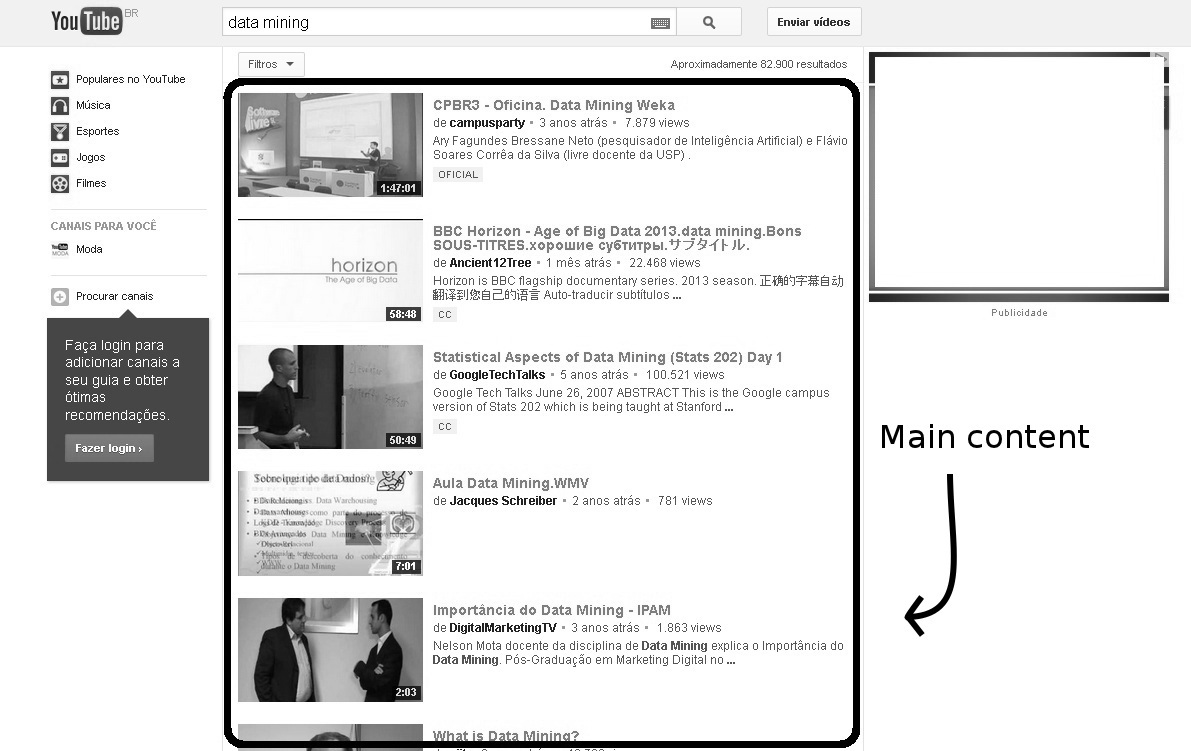
\includegraphics[scale=0.29]{example2-gs.jpg}
\end{figure}
}

\section{Related work} 
%\frame{\tableofcontents[currentsection]}
\frame{\frametitle{Related work} 
\begin{itemize}
	\item Text content based approaches (does not take page structure into consideration);
	\item DOM tree based approaches (classical representation of a web page);
	\item Visual information based approaches (huge overhead due to web page renderer dependency);
	\item Tag paths (string representation that retains structural information).
\end{itemize}
}

\frame{\frametitle{Related work}
\begin{tiny}
\begin{table}[h]
\centering
\caption{Comparative table of segmentation techniques}
\label{table:comp}
\begin{tabular}{l c c c c c}
\hline\hline
          &          &        &          & Needs       & HTML \\
          & Operates & Single & Training & a priori    & syntax \\ 
Technique & over     & page   &          & information & dependent \\
\hline
Fernandes et al. [2007] & Text & - & - & - & - \\
Kohlschütter and Nejdl [2008] & Text & - & - & - & - \\
Kohlschütter et al. [2010] & Text & - & - & - & - \\
Weninger et al. [2010] & Text & - & - & - & - \\
Hu et al. [2013] & Text & - & - & - & - \\
Yi et al. [2003] & DOM Tree & No & Yes & No & No \\
Chakrabarti et al. [2008] & DOM Tree & No & Yes & No & No \\
Cho et al. [2009] & DOM Tree & Yes & No & Yes & Yes \\
Fernandes et al. [2011] & DOM Tree & No & Yes & No & No \\
Zheng et al. [2012] & DOM Tree & Yes & No & Yes & Yes \\
Zheng et al. [2007] & DOM Tree & No & Yes & No & No \\
Cai et al. [2003] & Visual rep. & Yes & No & Yes & Yes \\
Simon and Lausen [2005] & Visual rep. & Yes & No & No & Yes \\
Liu et al. [2010] & Visual rep. & Yes & No & Yes & Yes \\
\hline
Our proposal & TPS & Yes & No & No & No \\
\end{tabular}
\end{table}
\end{tiny}
}


\subsection{Tag paths}

\frame{\frametitle{Tag paths}
\begin{figure}[H]
  \caption{An example of a TPS being built from an HTML code.}
  \label{fig:ex1}
  \centering
    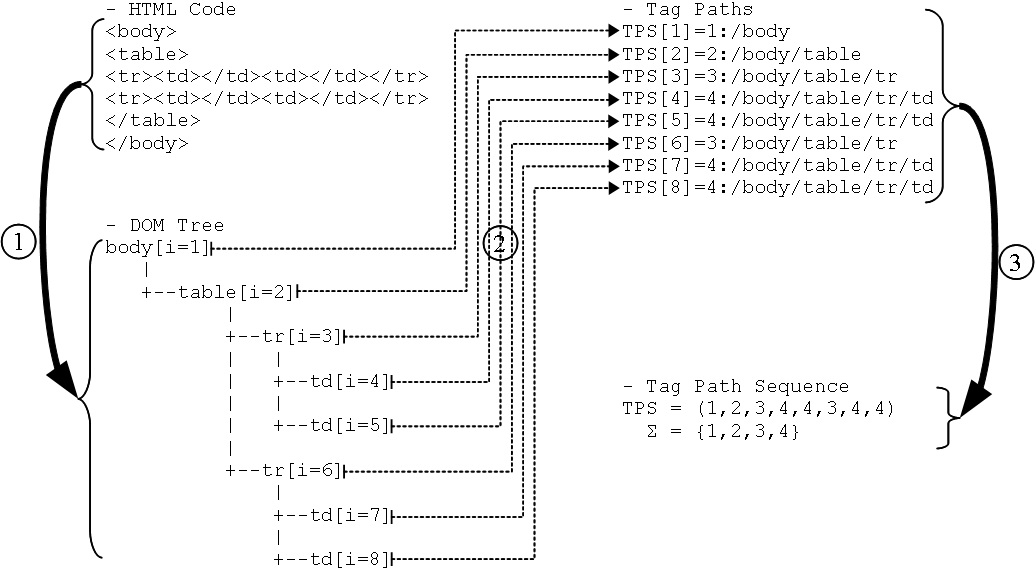
\includegraphics[scale=0.33]{example1.jpg}
\end{figure}
}
\section{Contributions} 
%\frame{\tableofcontents[currentsection]}
\frame{\frametitle{Contributions}
\begin{small} 
\begin{itemize}
\item{Fully automatic}: no training or human intervention involved;
\item{Domain independent}: it is only required that a page contains structured content, no matter what domain it is about;
\item{HTML syntax independent}: there are no rules defined for specific HTML tags; 
\item{Works on single page}: it is required only one page as input;
\item{Can be combined with extraction techniques}: due to the way pruning is carried out (preserving tree structure), this algorithm can be combined with any structured extraction algorithm;
\item{Extraction optimization}: the proposed algorithm prunes an average of 46.22\% of the DOM tree, avoiding the processing of this noise by the subsequent extraction algorithm.  
\end{itemize}
\end{small}
}
\section{Hypothesis} 
%\frame{\tableofcontents[currentsection]}
\frame{\frametitle{Hypothesis}

\begin{enumerate}
\item\label{ass:1}
different regions of a web page are described using different tag paths, so
these regions will have different alphabets; and
\item\label{ass:2}
in web sites with semi-structured content, the main region is structurally denser than the others (menus, ads,
text, etc.).
\end{enumerate}
}
\subsection{Algorithm}

\frame{\frametitle{Algorithm}
\begin{figure}[H]
  \caption{Algorithm illustration.}
  \label{fig:alg}
  \centering
    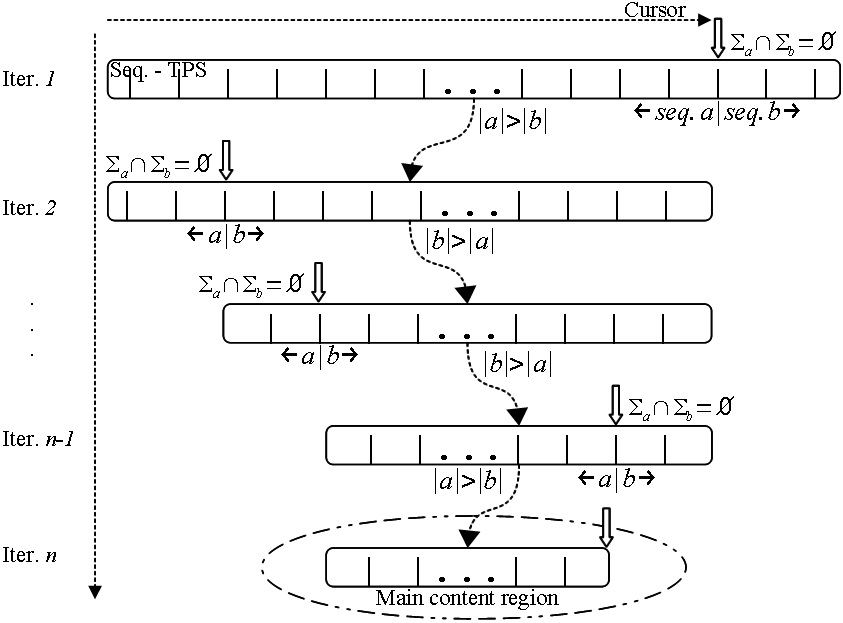
\includegraphics[scale=0.36]{alg-pb.jpg}
\end{figure}
}

\frame{\frametitle{Algorithm}
\begin{figure}[H]
  \caption{Detection of the main content region in a real web page.}
  \label{fig:alg}
  \centering
    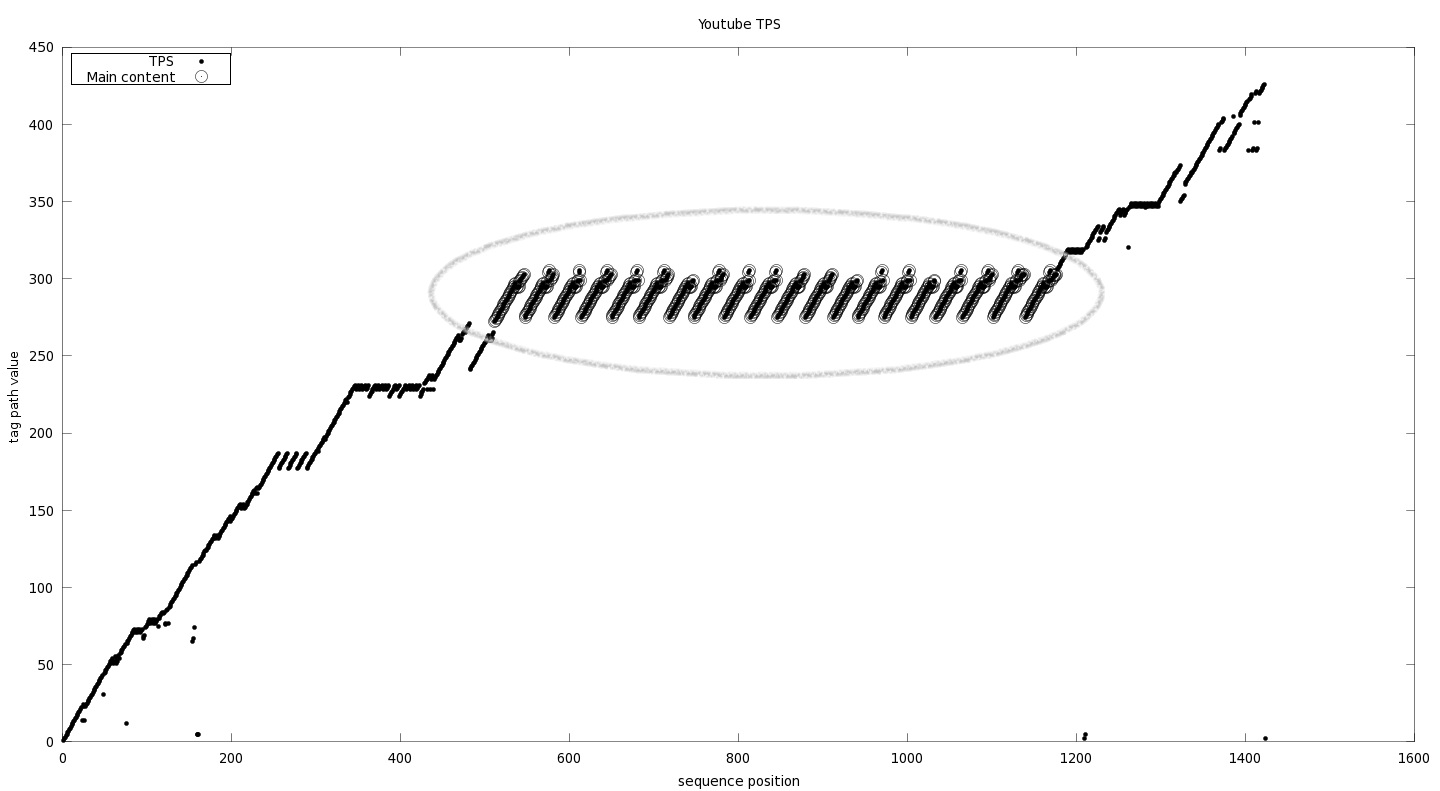
\includegraphics[scale=0.40]{tps.jpg}
\end{figure}
}

\begin{frame}[fragile]
\frametitle{Algorithm - filtering procedure}
\fontsize{8}{7.2}\selectfont
\begin{itemize}
\item{HTML code} 
\begin{verbatim}
<body>
<br>
<div>
  <span class='region1'></span>
  ...
  <span class='region1'></span>
</div> 
<div>
  <span class='region2'></span>
  ...
  <span class='region2'></span>
</div>
<div>
  <span class='region3'></span>
  ...
  <span class='region3'></span>
</div>
<br>
</body>
\end{verbatim}
\item{TPS}
\begin{verbatim}
TPS = (1,2,3,4,...,4,3,5,...,5,3,6,...,6,2)
\end{verbatim}
\item{Filtered TPS}
\begin{verbatim}
TPS = ( , , ,4,...,4, ,5,...,5, ,6,...,6, )
\end{verbatim}
\end{itemize}
\end{frame}

\section{Evaluation method} 
%\frame{\tableofcontents[currentsection]}
\frame{\frametitle{Evaluation method}
\begin{figure}[H]
  \caption{Evaluation method adopted.}
  \label{fig:alg}
  \centering
    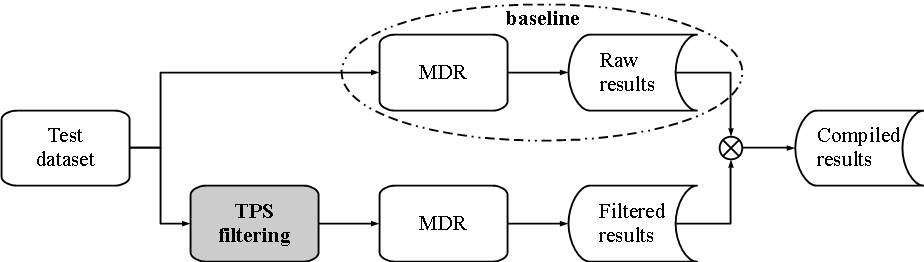
\includegraphics[scale=0.37]{method.jpg}
\end{figure}
}

\section{Results} 
%\frame{\tableofcontents[currentsection]}
\frame{\frametitle{Results} 
\begin{figure}[H]
  \label{fig:res}
  \centering
    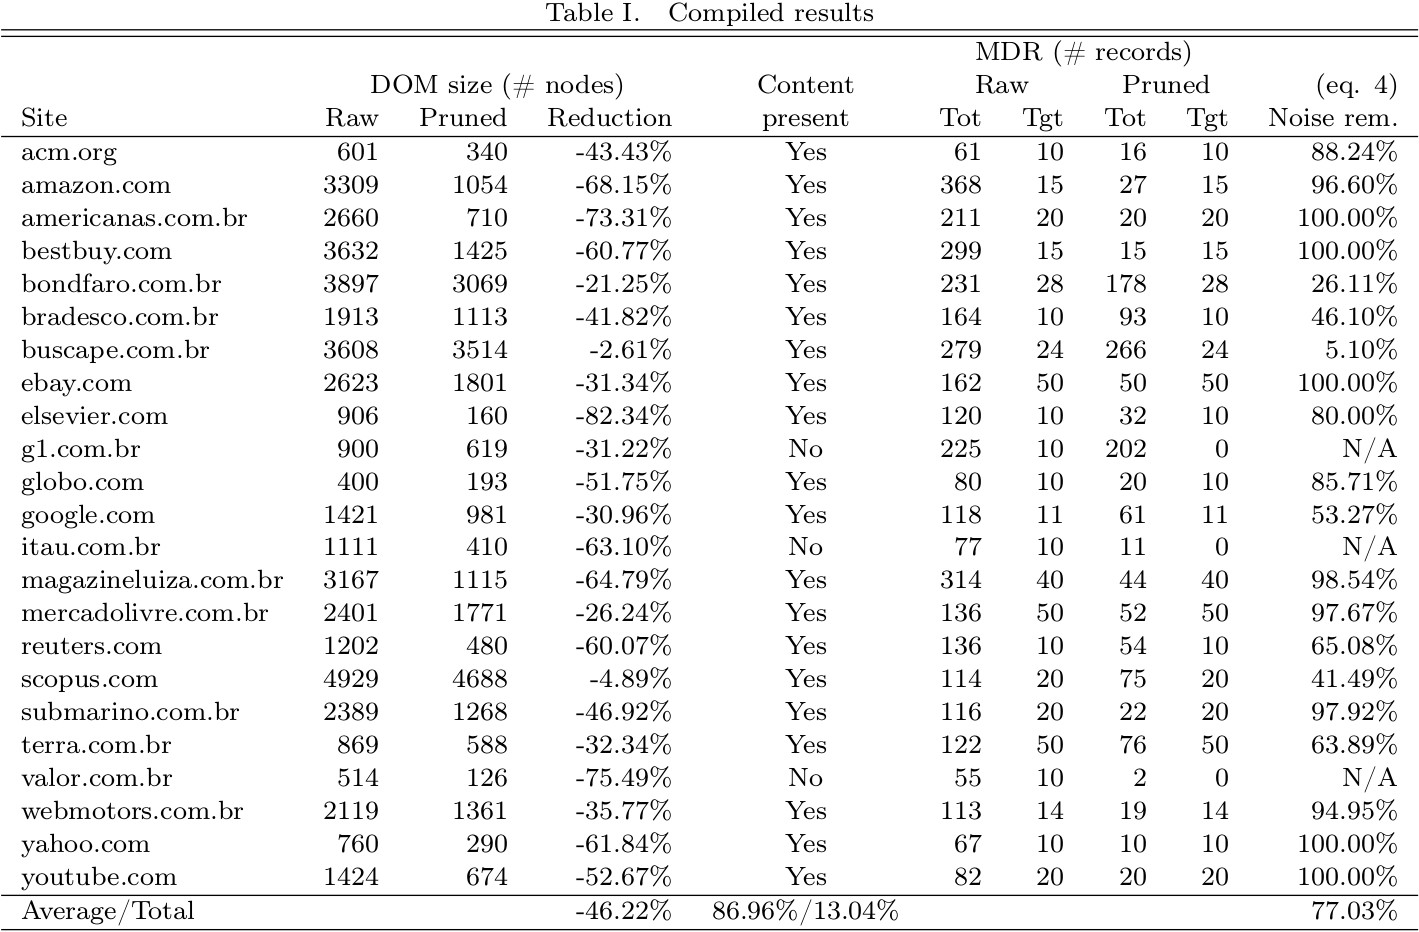
\includegraphics[scale=0.18]{result.jpg}
\end{figure}
}

\section{Limitations} 
%\frame{\tableofcontents[currentsection]}
\frame{\frametitle{Limitations}
\begin{enumerate}
  \item{templates too homogeneous};
  \item{templates too heterogeneous};
  \item{pages where the main content is smaller than the rest}.
\end{enumerate}
}

\section{Future work}
%\frame{\tableofcontents[currentsection]}
\frame{\frametitle{Future work}
\begin{itemize}
  \item Combine other approaches and techniques (semantic approaches);
  \item Propose a more general hypothesis about web pages with structured content. 
\end{itemize}
}

\end{document}
